\begin{question}
\noindent Triangle $A$ has vertices at $(-1, 1)$, $(-1, 3)$ and $(-3, 1)$.

\noindent On the grid below, enlarge triangle $A$ by scale factor $-2$, using $(1, 1)$ as the centre of enlargement. Label the image $A'$.

\begin{center}
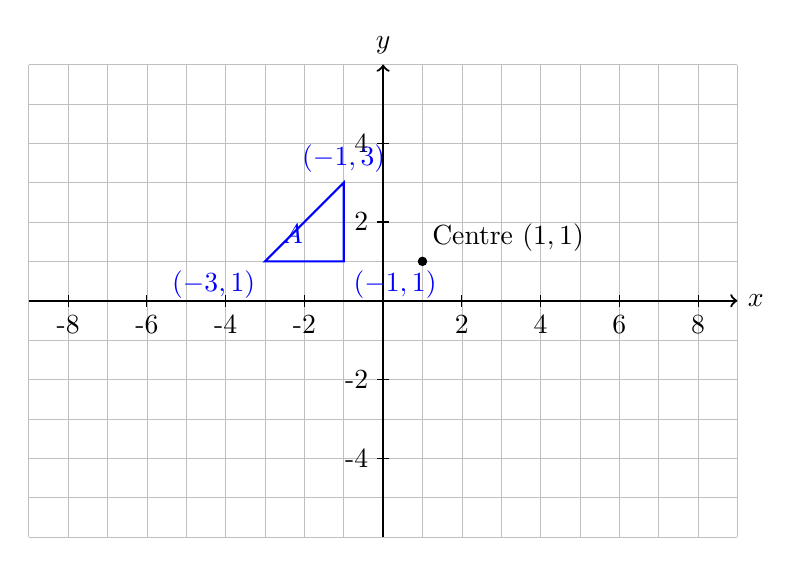
\begin{tikzpicture}[scale=0.5]
    \draw[step=1cm, lightgray, very thin] (-9,-6) grid (9,6);
    \draw[thick,->] (-9,0) -- (9,0) node[right]{$x$};
    \draw[thick,->] (0,-6) -- (0,6) node[above]{$y$};

    \foreach \x in {-8,-6,-4,-2,2,4,6,8}
        \draw (\x,-0.15) -- (\x,0.15) node[below=4pt]{\x};
    \foreach \y in {-4,-2,2,4}
        \draw (-0.15,\y) -- (0.15,\y) node[left=4pt]{\y};

    \draw[thick, blue] (-1,1) -- (-1,3) -- (-3,1) -- cycle;
    \node[blue] at (-1,1) [below right] {$(-1,1)$};
    \node[blue] at (-1,3) [above] {$(-1,3)$};
    \node[blue] at (-3,1) [below left] {$(-3,1)$};

    \node at (-2.3,1.7) [blue] {$A$};

    \filldraw[black] (1,1) circle (3pt);
    \node at (1,1) [above right] {Centre $(1,1)$};
\end{tikzpicture}
\end{center}

\vspace{6cm}
\answerplain{4}
\end{question}
